\documentclass[12pt]{article}
\usepackage[utf8]{inputenc}
\usepackage{geometry}
\PassOptionsToPackage{usenames,dvipsnames}{color}  %% Allow color names
\usepackage[svgnames]{xcolor}
\usepackage{framed}        % enable shading
\usepackage[hyphens]{url}  % wrap urls across lines, breaking by hyphens
\usepackage{hyperref}
\usepackage{listings}
\usepackage{float}         % keep figures in order
\usepackage{graphicx}      % allow graphics/figures
\usepackage{sectsty}       % set section header font sizes
\usepackage[compact]{titlesec}  % set skip after sections
\usepackage{enumitem}
\usepackage{amssymb}


\geometry{margin=1in}

% set up url
\hypersetup{
    colorlinks=true,
    linkcolor=blue,
    filecolor=magenta,      
    urlcolor=NavyBlue,
}

% color to shade with
\definecolor{shadecolor}{gray}{0.9}
\usepackage{tgpagella}

 %put box around figure captions
\makeatletter
\long\def\@makecaption#1#2{%
  \vskip\abovecaptionskip
  \sbox\@tempboxa{\fbox{#1: #2}}%
  \ifdim \wd\@tempboxa >\hsize
    \fbox{\parbox{\dimexpr\linewidth-2\fboxsep-2\fboxrule}{#1: #2}}\par
  \else
    \global \@minipagefalse
    \hb@xt@\hsize{\hfil\box\@tempboxa\hfil}%
  \fi
  \vskip\belowcaptionskip}
\makeatother

%no indent and modify distance between paragraphs
\setlength\parindent{0pt}
\setlength\parskip{12pt}

% Reduce spacing after section headers
\titlespacing{\section}{0pt}{*1}{*0}
\titlespacing{\subsection}{0pt}{*1}{*0}
\titlespacing{\subsubsection}{0pt}{*0}{*0}


\begin{document}

\begin{center}
{\Large \textbf{CS 330 2023 Homework 3} \\ Few-Shot Learning with Pre-trained Language Models
\\ 
\vspace{0.2cm}
Due Monday November 6th, 11:59 PM PT}

\begin{tabular}{rl}
SUNet ID: &  \\
Name: & Seok, Jeongeum\\
Collaborators: & 
\end{tabular}
\end{center}

By turning in this assignment, I agree by the Stanford honor code and declare that all of this is my own work.

\section*{Overview}
This assignment will explore several methods for performing few-shot (and zero-shot) learning with pre-trained language models (LMs), including variants of fine-tuning and in-context learning. The goal of this assignment is to gain familiarity with performing few-shot learning with pre-trained LMs, learn about the relative strengths and weaknesses of fine-tuning and in-context learning, and explore some recent methods proposed for improving on the basic form of these algorithms.

\noindent We have provided you with starter code, which can be downloaded from the course website.

\textbf{Submission:} To submit your homework, submit one PDF report to Gradescope containing written answers and Matplotlib plots (screenshots are acceptable) to the questions below, as well as a single zip file containing:
\begin{itemize}
    \item \texttt{\_\_init\_\_.py}
    \item \texttt{ft.py}
    \item \texttt{icl.py}
    \item \texttt{results}
\end{itemize}
\textbf{Note: the autograder will only work if all these files are contained in the root of the zip!} I.e. not inside a subdirectory.

 The PDF should also include your name and any students you talked to or collaborated with. \textbf{Any written responses or plots to the questions below must appear in your PDF submission.}

\textbf{Setup:} This assignment requires using the HuggingFace library for loading pre-trained models and datasets. The required packages are provided in a \texttt{requirements.txt} file to enable easy installation, which you can install using \texttt{pip install -r requirements.txt}. If you have trouble installing on your laptop (e.g. some Apple Silicon machines), you can use your Azure instance to debug. If you're having trouble installing the requirements, you might need a specific CUDA version; checking the \href{https://pytorch.org/get-started/locally/}{PyTorch install guide} might help find the right version.

\textbf{Code Overview:} The code consists of several files to enable fine-tuning and in-context learning. You are expected to write the code in the following files:
\begin{itemize}
    \item \texttt{ft.py}: Fine-tuning script; you'll implement parameter selection, loss \& accuracy calculation, the LoRA implementation (this will be explained in Q2!), fine-tuning batch tokenization, and the model update step.
    \item \texttt{icl.py}: In-context learning script; you'll implement prompt assembly and model sampling.
\end{itemize}

You only need to change these two files. A detailed description for every function can be found in the comments. You are not expected to change any code except for sections marked with \texttt{YOUR CODE HERE}.

\textbf{Please complete questions in order}, since they depend on previous components.

\section*{Compute}

For this assignment, you will complete all sections on Azure instances with GPUs. Avoid using Azure for debugging; verify that your code runs without crashing on your own machine, and use Azure only once you think your code is finished.

The \href{https://docs.google.com/document/d/1wm2m6gQtxgxXV5V7UUDUVOktJjOF_vzxJt29fdn8M5E/edit}{CS330 Azure Guide} has instructions for setting up and accessing an Azure GPU spot instance.

{
\begin{center}
\large
    \textbf{\textit{Be sure to shut down your Azure instance when not in use!}}
\end{center} 
}

\section*{Datasets}

You'll explore three different language datasets in this assignment. The first, Amazon Reviews, is a classification dataset that you'll use for the warmup. The other two, XSum and bAbI, require generating open-ended language.

\begin{enumerate}
    \item For the fine-tuning warmup, we'll explore a simple text classification problem, a subset of the \href{https://huggingface.co/datasets/amazon\_us\_reviews}{Amazon Reviews} dataset. The portion of the Amazon Reviews dataset that we will consider contains paired video reviews and star ratings; the task we will consider will be five-way classification of a review into the number of stars its corresponding rating gave, among \texttt{\{1,2,3,4,5\}}. \textbf{You can expect accuracy numbers \textit{roughly} in the 0.2-0.4 range for Amazon Reviews in this assignment.}
    \item \href{https://huggingface.co/datasets/xsum}{XSum}: The XSum dataset contains news articles from the BBC and corresponding one sentence summaries. The evaluation metric typically used for summarization is \textbf{\href{https://en.wikipedia.org/wiki/ROUGE_(metric)}{ROUGE} score}, which measures $n$-gram overlap between the target and prediction (how many words appear in both, how many bigrams, etc.). An \href{https://en.wikipedia.org/wiki/N-gram#Examples}{$n$-gram} is a subsequence of $n$ consecutive words, in this context.  \textbf{You can expect ROUGE scores \textit{roughly} in the 0.1-0.3 range for XSum in this assignment.}
    \item \href{https://research.facebook.com/downloads/babi/}{bAbI} is a AI benchmark suite developed by Facebook AI Research. The task that we will use is a question-answering task that requires reasoning about contextual information that may or may not be relevant to answer a question. A sample question from the dataset is:
    
    \texttt{Mary went back to the office. John went to the bathroom. Where is Mary? In the office}
    
    \textbf{You can expect accuracy numbers \textit{roughly} in the 0.25-0.9 range for bAbI QA in this assignment.}
\end{enumerate}

These datasets, except for the Amazon Reviews dataset are available through the HuggingFace library.

\vspace{0.2cm}
\noindent\textbf{Optional. Autograding Your Code.}
In this homework, we include autograding functionalities in the released code to facilitate you to debug and develop your code. To run the autograder, simply do:

\texttt{python grader.py}

\noindent The maximum points you can get when running the autograder is \textbf{14 / 14 points}. We also have \textbf{36 points} from hidden test cases that show up when you submit your code to Gradescope. This makes the total of \textbf{50 points} for all the coding parts.

\section*{(10 pt) Question 0: Fine-tuning warmup}
As a warmup, we will perform perhaps the most straightforward form of $k$-shot learning with a pre-trained model: directly fine-tuning the entire model on the $k$ examples. We will use two different sizes of smaller BERT models that have been compressed through distillation.\footnote{See \href{https://arxiv.org/pdf/1908.08962.pdf}{here} to learn more about this class of distilled BERT models. For final projects involving language models, these smaller BERT models may be useful for performing compute-friendly experiments!}

\begin{enumerate}
    \item Implement the logic for fine-tuning, including selecting the parameters that will be fine-tuned (only the case for \texttt{`all'} for this question) in \texttt{ft.py:\allowbreak parameters\_to\allowbreak \_fine\_tune()}, and computing the loss and accuracy in \texttt{ft.py:\allowbreak get\_loss} and \texttt{ft.py:\allowbreak get\_acc}. You only need to complete the loss/accuracy calculations under \texttt{if logits.dim() == 2:} for this question.
    \item The Amazon Reviews dataset is no longer available through HuggingFace, so we are providing an adapted version of the Kaggle dataset to \href{https://drive.google.com/file/d/1RLCPCEvJVTvUbn-D426Avwg6hynSBgU3/view?usp=sharing}{download here}. Please place the \textit{uncompressed} csv file inside the \texttt{data} directory. You can run this command to send the file to your Azure instance:

    {
    \small\texttt{
    scp ~/Downloads/amazon\_reviews\_us\_Video\_v1\_00.csv azureuser@{instance\_public\_ip\_address}:$\small\sim$/
    }
    }
    \item (8 pt) Run the command:
    
    {\small\texttt{
    python ft.py --task ft --model bert-tiny,bert-med --dataset amazon --k 1,8,128
    }}
    
    to fine-tune two sizes of BERT models on the Amazon Reviews dataset for various values of $k$. While debugging, you can pass only one value for each of the arguments to run only that subset, e.g. \texttt{python ft.py --task ft --model bert-tiny --dataset amazon --k 1}.
    
    If you see a log message like \texttt{Some weights of the model checkpoint...}, this is expected, since the pre-trained model does not contain a prediction head for our task (this is why we need to fine-tune!).

    To plot your results, run the command:
    
    {\small\texttt{
    python ft.py --task plot --model bert-tiny,bert-med --dataset amazon --k 1,8,128 --plot\_name Q0\_3.png
    }}
    
    In one sentence, what do you notice about the performance of the two model scales?\\
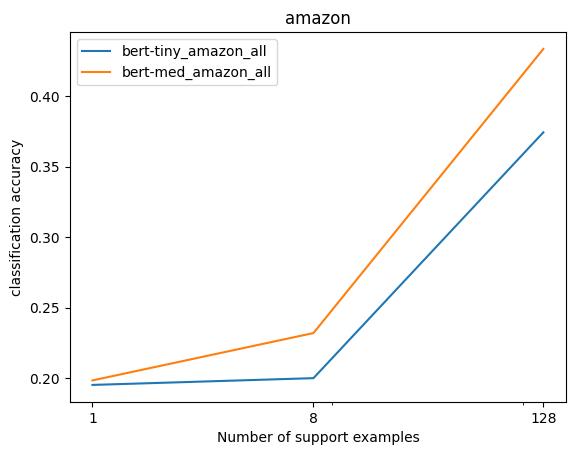
\includegraphics[width=\linewidth]{hw3_starter_code/starter_code/Q0_3.png}    
    \textbf{\color{red}Performance gets better with the bigger model and more support examples.}
    \item (1 pt) If we fine-tune the all of our model parameters for each task, we must save a new complete copy of the model's parameters for each new task. As an example, a BERT-mini model similar to the ones you just fine-tuned has approximately 11.2 million parameters; assuming parameters are represented as 4-byte floats, after fine-tuning on a new task, how much disk space do we need to store the new fine-tuned model parameters?

    \textbf{\color{red}44,800,000 bytes or 42.7 megabytes.}

    \item (1 pt) Google's recent large language model \href{https://storage.googleapis.com/pathways-language-model/PaLM-paper.pdf}{PaLM} has 540 billion parameters. How much disk space would be needed to store a new fine-tuned version of this model, assuming parameters are represented as 4-byte floats?

    \textbf{\color{red}1.96 terabytes.}

\end{enumerate}

\section*{(15 pt) Question 1: In-context learning}
A surprising property of large language models is their emergent ability to learn \textit{in-context}, that is, their ability to learn a task without updating any parameters at all. The name `in-context' comes from the fact that the learning is done by simply including several examples or a task description (or both!) prepended to a test input present to the model

For example, for a question-answering task, to make a 2-shot prediction for a test input `Why is the sky blue?', rather than presenting the input:

\texttt{Why is the sky blue?\textless generate\textgreater}

we would simply prepend our 2 examples to the input:

\texttt{Who is the US president? Joe Biden What is earth's tallest mountain? Mount... \\
Everest Why is the sky blue?\textless generate\textgreater}

In addition to few-shot in-context learning, models can often improve their zero-shot generalization if the input is formatted in a particular manner; for example, adding a \texttt{Q:} and \texttt{A:} prefix to the input and label, respectively:

\texttt{Q: Why is the sky blue? A:\textless generate\textgreater}

Finally, these two approaches can be combined, for example adding the \texttt{Q:} and \texttt{A:} markers to each example in the context as well as the test input.

\begin{enumerate}
    \item Complete the code for in-context learning in \texttt{icl.py}.
    \begin{enumerate}
        \item Implement prompt creation for the XSum and bAbI tasks, which is found in \texttt{icl.py:get\_icl\_prompts()}. Shuffle the order of the support inputs and targets, but preserving the pairings of input/labels. You will implement 4 prompt format modes:
        \begin{enumerate}
            \item \texttt{qa} \textbf{[only for bAbI]}: Add ``\texttt{ In the }'' after the question (including the final test question that we want to generate an answer for!) and before each answer, since this task involves answering questions about the physical whereabouts of a person. In addition, add a period after the answer (omitting the period can significantly impact your results!). Be sure to include a space between the question and \texttt{In the}, as well as a space before the answer (though keep in mind Note 1!). You do not need to add the "Q: A:" from the earlier example.
            \item \texttt{none} \textbf{[only for XSum]}: In this case, we use the raw $k$ examples without any additional formatting; that is, we just concatenate $[x_1; y_1; ... ; \allowbreak x_k; y_k; x^*]$ with a space between each element (but no space at the end), where $x^*$ is the input that we want to generate an answer for.
            \item \texttt{tldr} \textbf{[only for XSum]}: Add the text ``\texttt{ TL;DR: }'' after each article/input (including the final test article) and before the summary/target. Also add a space between each summary and the next article (but no space at the end).
            \item \texttt{custom} \textbf{[only for XSum]}: Come up with your own prompt format for article summarization (different from the ones we've shown!).
        \end{enumerate}
        In general, the idea of in-context learning is to format the support examples in the same way as the test example, to leverage the model's tendency toward imitation.

        Examples for the first 3 prompt types are available in the starter code.

        \textbf{Note 1: Due to a quirk with GPT-2 tokenization, you should not include a space at the end of your prompt before generation.}
        
        \textbf{Note 2: Be sure to shuffle the order of the support inputs/targets when you construct the prompt (we will need this randomization later).}
        \item Implement greedy sampling in \texttt{icl.py:do\_sample()}. The GPT-2 models used in this and the following questions use an autoregressive factorization of the probability of a sequence, i.e. $p_\theta(\mathbf{x}) = \prod_t p_\theta(x_t|x_{<t})$. `Greedy' sampling means that given a context $x_{<t}$ producing a distribution over next tokens $p_\theta(x_t|x_{<t})$, we deterministically choose the next token $x_t$ to be the token with highest probability. The documentation for the GPT-2 model used (\href{https://huggingface.co/docs/transformers/model_doc/gpt2#transformers.GPT2LMHeadModel}{transformers.GPT2LMHeadModel}) will be helpful. You should use caching to speed up generation and decrease memory usage.

        \emph{Tips to avoid out-of-memory errors:} Wrap calls to the model with \texttt{torch.inference\_mode()} (see \href{https://pytorch.org/docs/stable/generated/torch.inference_mode.html}{example here}). Also see the \texttt{past\_key\_values} and \texttt{use\_cache} arguments for the \texttt{GPT2LMHeadModel} model.
        
        \textbf{Note 3: Be sure you understand what each dimension of the model's output \texttt{logits} represents. Misinterpreting the dimensions of this output can lead to subtle bugs.}
        
        \item Finally, put the pieces together by completing the implementation of \texttt{icl.py:\allowbreak run\_icl()}, using your \texttt{get\_icl\_prompts()} and \texttt{do\_sample()} functions, as well as the HuggingFace tokenizer defined in the loop. \\ \emph{Hint}: Your solution here should be 5-10 lines of code.
    \end{enumerate}

    \item (10 pt) First, evaluate $k$-shot in-context performance on bAbI for GPT-2-medium (355M parameters) and full-size GPT-2 (1.5B parameters) for various values of $k$ with the command:
    
    \texttt{\small python icl.py --task icl --model med,full --dataset babi --k 0,1,16}
    
    Plot the results with the command:
    
    \texttt{\small python icl.py --task plot --model med,full --dataset babi --k 0,1,16 --plot\_name Q1\_2.png}
    
    What relationship(s) do you notice between model scale and few-shot performance?
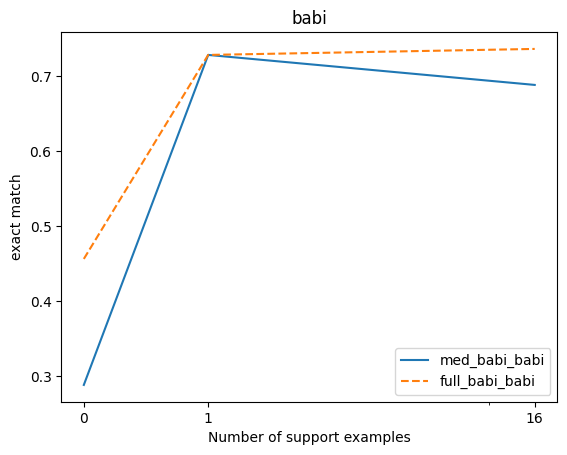
\includegraphics[width=\linewidth]{hw3_starter_code/starter_code/Q1_2.png}            
    \textbf{\color{red}The bigger model has robust few-shot performance.}

    \item (5 pt) Now let's evaluate several different prompt formats on the XSum dataset. With and without a task description in the prompt, evaluate zero-shot and few-shot performance for XSum on GPT-2-Medium with the command:

    \texttt{\small python icl.py --task icl --model med,full --dataset xsum --k 0,1,4 \textbackslash \\
    \phantom{asdf}--prompt none,tldr,custom}
    
    Note that we use much smaller $k$ than in the previous problem, because we must fit all $k$ examples into the model's context window, which is only 1024 tokens. The fixed context window length is one limitation of in-context learning.
    
    \textbf{The $k=4$ XSum evaluation on full-size GPT-2 may take approximately 40 minutes on your Azure instance for each prompt mode}; this is expected, and is another downside of in-context learning (we need to process a much longer input, containing the prompt, compared to a fine-tuned model that just processes the test input).
    
    Plot the zero-shot and few-shot performance of GPT-2 on XSum:
    
    \texttt{\small python icl.py --task plot --model med,full --dataset xsum --k 0,1,4 \textbackslash \\
    \phantom{asdf}--prompt none,tldr,custom --plot\_name Q1\_3.png}
    
    How does the performance of the \texttt{TL;DR:} prompt compare with no prompt formatting? What was your custom prompt format, and how did it compare with \texttt{TL;DR:}? Discuss the relative performance of the different prompts in the zero-shot, one-shot, and few-shot settings.
    
    \textbf{\color{red}Include your plot and answer here.}

\end{enumerate}

\section*{(15 pt) Question 2: Parameter-efficient fine-tuning}
As we observed in question 1, fine-tuning the entire model can become extremely costly for very large models. In this question, we'll explore more methods for \textit{parameter-efficient fine-tuning}, i.e., methods that enable fine-tuning while creating fewer new parameters and are less prone to overfitting.
\begin{enumerate}
    \item Finish the implementation for each version of parameter-efficient fine-tuning for GPT-2-Medium in \texttt{ft.py:parameters\_to\_fine\_tune()}:
    \begin{enumerate}
        \item \texttt{last}: Fine-tune only the last 2 transformer blocks
        \item \texttt{first}: Fine-tune only first 2 transformer blocks
        \item \texttt{middle}: Fine-tune only middle 2 transformer blocks
    \end{enumerate}
    This step simply requires selecting the correct subset of parameters for each version listed above in \texttt{parameters\_to\_fine\_tune()}. Keep in mind you should be returning an iterable of \texttt{nn.Parameter} here, not \texttt{nn.Module}.

    \emph{Hint}: to understand how to get parameters for specific layers, we encourage you to print the model architecture. You can place a Python debugging breakpoint anywhere in the code with `\texttt{import pdb; pdb.set\_trace()}`, and can run the command in subpart 3 to get the function to run with the right parameters.

    \item In addition to selecting only a subset of layers to fine-tune, more sophisticated methods for parameter-efficient fine-tuning exist; one such method is \href{https://arxiv.org/pdf/2106.09685.pdf}{LoRA: Low-rank adaptation}. For each layer $\ell$ in the network, rather than fine-tune the pre-trained weight matrix $W_\ell^0 \in \mathbb{R}^{d_1\times d_2}$ into an arbitrary new weight matrix $W_\ell^{ft}$, LoRA constrains the space of fine-tuned parameters such that $W_\ell^{ft} = W_\ell^0 + AB^\top$, where $A \in \mathbb{R}^{d_1\times p}$ and $B \in \mathbb{R}^{d_2\times p}$, and $p << d_1,d_2$. That is, we force the \textit{difference} between $W_\ell^0$ and $W_\ell^{ft}$ to be rank $p$, keeping $W_\ell^0$ frozen and only fine-tuning the rank-$p$ residual matrix $AB^\top$. We will apply this form of fine-tuning to both the MLP weight matrices and the self-attention weight matrices in the model.
    \begin{enumerate}
        \item For a single layer, what are the parameter savings we achieve by using LoRA? i.e., what is the ratio of parameters fine-tuned by LoRA (for arbitrary $p$) to the number of parameters in $W_\ell^0$? In terms of $p,d_1,d_2$, when will LoRA provide the greatest savings in newly-created parameters?
        \item Finish the \texttt{LoRALayerWrapper} in \texttt{ft.py}, which wraps a pre-trained linear layer with LoRA parameters. You can extract the shape of the pre-trained weight matrix from the \texttt{base\_module.weight.shape} tuple. You don't need to worry about biases here, just the low-rank weight matrix residual.
        
        \item Add the corresponding logic for LoRA in \texttt{ft.py:parameters\_to\_fine\_tune()}. Hint: consider using the \texttt{.modules()} function of \texttt{nn.Module} and checking for modules that are an instance of \texttt{LoRALayerWrapper}.
        \item Implement the 3-dim version of the loss and accuracy in \texttt{ft.py:get\_loss()} and \texttt{ft.py:get\_acc()}.
        \item Implement batch construction for fine-tuning GPT-2 in function \texttt{ft.py:\allowbreak tokenize\_\allowbreak gpt2\_batch()}. Read the instructions in the code carefully!
        \item Finally, put it all together by filling out the logic for one step of training in \texttt{ft.py:ft\_gpt2()}. Note that we use \textit{gradient accumulation}, meaning that accumulate gradients over \texttt{grad\_accum} steps, and only update our model's parameters after each \texttt{grad\_accum} steps.
    \end{enumerate}
    
    \item (15 pt) Run fine-tuning for each parameter-efficient fine-tuning method, using $p=4,16$ for LoRA (so, 5 variants in total); run the commands:

    {\small \texttt{python ft.py --task ft --model med --mode first,last,middle,lora4,lora16 \textbackslash \\
    \phantom{asdf}--dataset xsum,babi --k 0,1,8,128}}

    Plot \textbf{k-shot performance} as \textbf{k is varied} for GPT-2-medium, one plot for each dataset; run the commands:

    {\small \texttt{python ft.py --task plot --model med --mode first,last,middle,lora4,lora16 \textbackslash \\
    \phantom{asdf}--dataset xsum --k 0,1,8,128 --plot\_name Q2\_3\_xsum.png}}

    {\small \texttt{python ft.py --task plot --model med --mode first,last,middle,lora4,lora16 \textbackslash \\
    \phantom{asdf}--dataset babi --k 0,1,8,128 --plot\_name Q2\_3\_xsum.png}}
    
    \textbf{\color{red}Include your plots and describe the results here.}

\end{enumerate}

\section*{(10 pt) Question 3: Comparing in-context learning and fine-tuning}

\begin{enumerate}
    \item (5 pt) Plot the few-shot performance of LoRA-16 and in-context learning for XSum in the same plot with the command:

    {\small\texttt{python q3\_plot.py}}

    When does in-context learning seem like the better choice, with respect to the amount of data available? What about fine-tuning? What limitation of in-context learning does this result highlight?
    
    \textbf{\color{red}Include your plot and write your answer here.}

    \item (5 pt) One potential disadvantage of in-context learning is that we must choose an ordering for the examples in our prompt, and \textit{that ordering can sometimes impact performance negatively}. Run the command:

    {\small \texttt{python icl.py --task icl --model med --dataset babi --k 16 --repeats 5}}

    to compute the evaluation performance of in-context few-shot performance for 5 random orderings of the prompt. Report the number you get; the standard deviation of performance for fine-tuning is approximately 0.013. Does in-context learning or fine-tuning have a higher standard deviation?
    
    \textbf{\color{red}Write your answer here.}

    \textbf{(5 pt) Extra credit:} See \href{https://arxiv.org/pdf/2104.08786.pdf}{this paper} for multiple heuristics for picking a prompt ordering. Implement either the globalE or localE heuristic, and report the accuracy you find for that ordering for 16-shot bAbI on GPT-2-medium. Compare it with the accuracy you found with random prompt orderings in question 1.
    
    \textbf{\color{red}Write your answer here.}
\end{enumerate}


\end{document}


